\chapter{Conceptos previos}\label{conceptosprevios}

%
%   GRUPOS FINITOS
%

\section{Grupos finitos}

Los grupos finitos cíclicos y los módulos se tratan mucho en criptografía, sin embargo, la notación matemática puede ser un poco liosa. Es por esto que incluimos esta sección entre los conceptos previos.

\begin{itemize}
    \item $\mathbb{Z}/n\mathbb{Z}$ es un grupo cíclico de $n$ elementos enteros.
\end{itemize}

En concreto, nosotros vamos a tomar $n = p$ donde $p$ es primo, por lo que este \textit{grupo} cíclico es equivalente al \textit{cuerpo} cíclico

\begin{itemize}
    \item $\mathbb{F}_p$ es un cuerpo cíclico de $p$ elementos.

    \item $\mathbb{F}_{p^2}$ es un cuerpo complejo de $p^2$ elementos con la siguiente forma 
        \[ \mathbb{F}_{p^2} = \mathbb{F}_{p}(i) = \{ u + vi : u,v \in \mathbb{F}_{p} \} \]
\end{itemize}

Un grupo es la combinación de un conjunto de elementos (cualquier elemento, podría ser números naturales, reales o puntos en un plano) junto con una operación suma. Un cuerpo, sin embargo, amplía el grupo con una operación multiplicación.  Estas operaciones no tienen por qué comportarse como las operaciones suma y multiplicación que conocemos pero sí que suelen mantener el mismo nombre y propiedades. Un cuerpo es mucho más robusto que un grupo y permite una mayor flexibilidad a la hora de trabajar con él. 

\subsection{Puntos de torsión}

Un elemento $g$ de un grupo finito $G$ se denomina de torsión si tiene orden finito. Esto es, si existe un entero $z$ tal que $g^z = e$ elemento neutro del grupo\footnote{Esta operación se corresponde a la operación multiplicación. En el caso de que el grupo sea una curva elíptica, se cumple que $z \cdot g = e$ donde $z$ es un entero y $e$ es el elemento neutro}. Decimos entonces de $g$ que es un punto de $z$-torsión del grupo.

Además, en las condiciones en las que vamos a trabajar, los puntos de torsión de un orden determinado forman un subgrupo. Este subgrupo tendrá forma $\mathbb Z_t \times \mathbb Z_t$ donde $t$ es el orden de torsión de los elementos siempre y cuando este $t$ sea coprimo con el primo seleccionado. Se cumple también, que cada uno de estos puntos de torsión junto con el infinito serán generadores de subgrupos cíclicos del orden correspondiente, siempre que $t,p$ sean coprimos.


%
%   CURVAS ELIPTICAS
%

\section{Curvas elípticas}

Una curva elíptica se definen mediante ecuaciones de tercer grado a las que usualmente se le añade un punto postizo que equivale al infinito. Una misma curva elíptica puede tener varias ecuaciones debido a la forma de estructurar la propia ecuación. Estas formas son equivalentes y las podemos calcular mediante cambios de variables.

Nosotros trataremos dos formas principales, la de Weierstrass \cite{jinvariant} y la de Montgomery, que definimos a continuación.

\begin{theorem}[Forma de Weierstrass]
Una curva elíptica es una curva de la forma
\[y^2 = x^3 + a \cdot x + b \]
donde los valores de $a,b$ cumplen la siguiente condición
\[ a^3-27 \cdot b^2 \neq 0 \]
\end{theorem}

\begin{theorem}[Forma de Montgomery]
Una curva elíptica es una curva de la forma
\[b \cdot y^2 = x^3 + a \cdot x^2 + x \]
donde los valores de $a,b$ cumplen la siguiente condición
\[ b \cdot (a^4 - 4) \neq 0 \]
\end{theorem}

\begin{figure}[h]
    \centering
    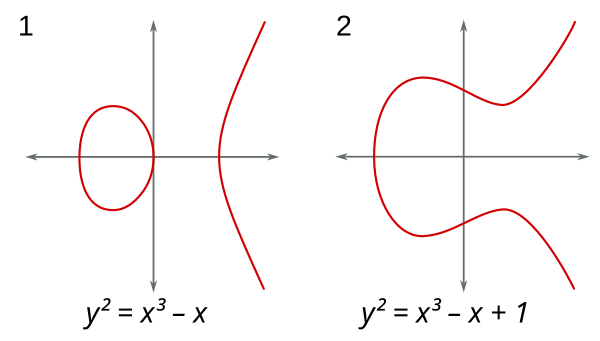
\includegraphics[width=0.5\linewidth]{img/curvas.png}
    \caption{Ejemplo de curvas elípticas}
    \label{fig:curvas}
\end{figure}

\subsection{Curvas elípticas sobre cuerpos finitos}

Nosotros no vamos a tratar sobre curvas continuas como son las que acabamos de ver sino con curvas definidas sobre cuerpos finitos, en concreto cuerpos del tipo $\mathbb F_{p^2}$. Estas curvas son visualmente bastante diferentes a las típicas gráficas a las que estamos acostumbrados, correspondiéndose más adecuadamente a una nube de puntos que a la línea continua que acabamos de ver.

\begin{figure}[h]
        \centering
    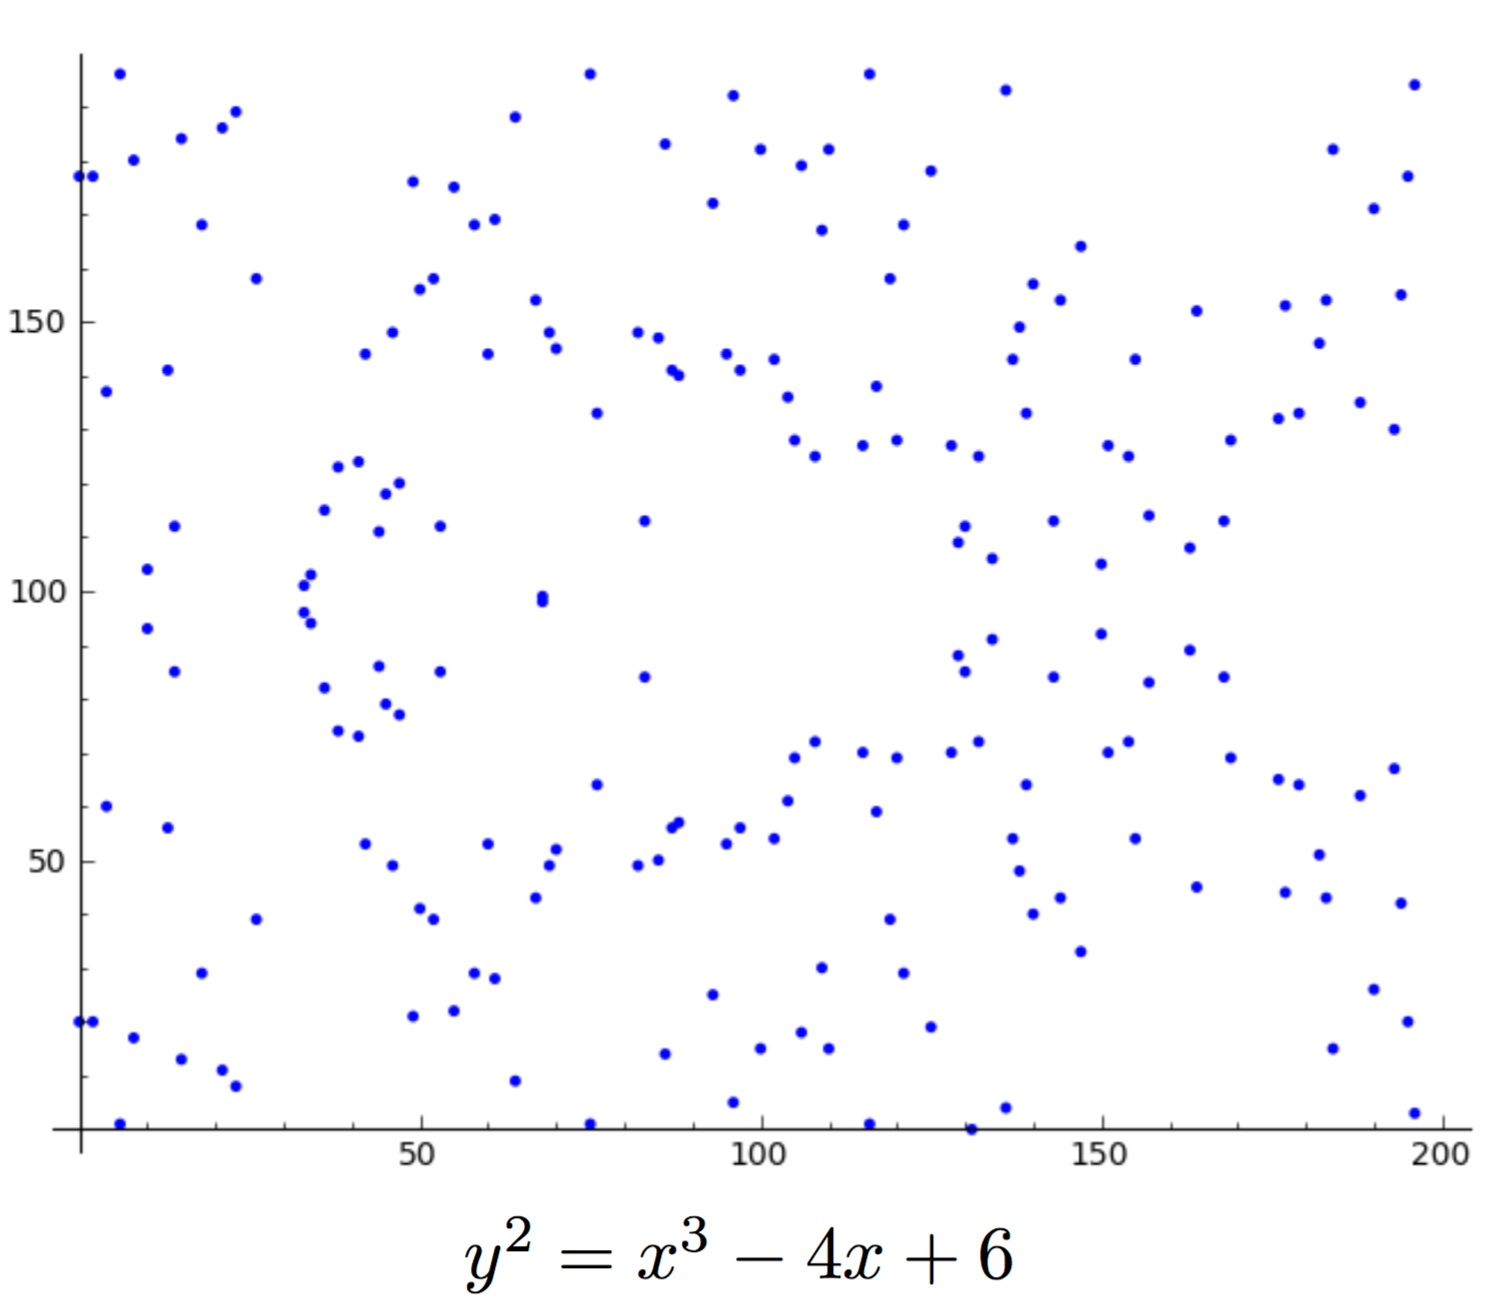
\includegraphics[width=0.7\linewidth]{img/curva-eliptica-finita.jpg}
    \caption{Curva elíptica definida sobre un cuerpo finito}
    \label{fig:curva-eliptica-finita}
\end{figure}

Sabiendo la composición de nuestro primo, que siempre va a ser de la forma $p=l_A^{e_A}l_B^{e_B}f \pm 1$ donde $l_A,l_B$ son primos pequeños\footnote{En concreto, estos primos pequeños serán $l_A=2,l_B=3$ ya que la diferencia en seguridad con primos más grandes no es tanta para la diferencia en velocidad que estos valores ofrecen.} sabemos que cualquier curva $E$ definida sobre el cuerpo $\mathbb F_{p^2}$ va a tener cardinalidad $(l_A^{e_A}l_B^{e_B}f)^2$.  A partir de aquí definimos el conjunto $E[l_A^{e_A}]$ que contiene a los $l_A^{e_A-1}(l_A+1)$ subgrupos cíclicos de orden $l_A^{e_A}$. Se construye el conjunto $E[l_B^{e_B}]$ de manera análoga.


\subsection{Curvas elípticas como grupos}

Como mencionamos en la sección anterior, los elementos de un conjunto pueden ser de la naturaleza que uno quiera. En este caso, vamos a tratar el conjunto de los puntos de una curva elíptica determinada.

Además de establecer este conjunto, las usaremos como grupo. Para ello, tenemos que definir previamente las operaciones que utilizaremos como operación de suma y multiplicación.

\subsubsection{Operación suma}

Dados dos puntos $P,Q \in E$, llamamos $L$ a la recta que une a estos dos puntos. Esta recta corta a la curva $E$ en un tercer punto $T$. Hacemos una segunda recta $L'$ que conecta el punto $T$ con el punto infinito $O$. $P+Q$ es, entonces, el tercer punto en el que la recta $L'$ intersecta a la curva $E$. En el caso de querer calcular el doble de un punto, la recta resultante será la tangente a la curva que pasa por ese punto. En las figuras \ref{fig:suma-distintos} y \ref{fig:suma-doble} incluimos ejemplos gráficos de la operación suma.

\begin{figure}[h]
    \centering
    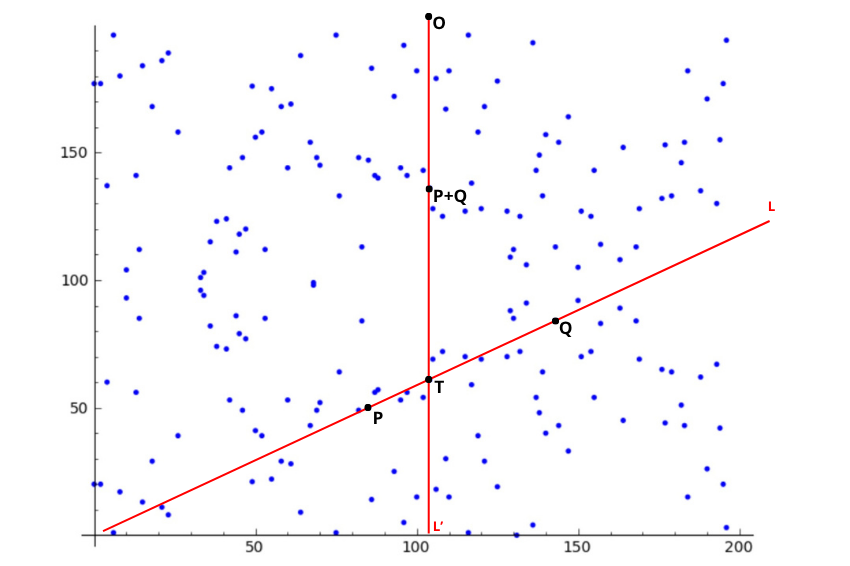
\includegraphics[width=0.7\linewidth]{img/suma.png}
    \caption{Operación suma para las curvas elípticas}
    \label{fig:suma-distintos}
\end{figure}


\subsection{Curvas elípticas supersingulares}

Tal y como dice el nombre del protocolo, SIKE no utiliza cualquier curva elíptica sino que se centra en aquellas denominadas supersingulares. Las curvas elípticas se dividen en las \textit{ordinarias} y las \textit{supersingulares}.

No vamos a entrar en mucho detalle en la definición de curva supersingular ya que implica un nivel de complejidad y formalidad demasiado alto. \footnote{Para profundizar en el tema, se puede consultar el artículo \textit{An Introduction to Supersingular Elliptic Curves  and Supersingular Primes} \cite{intro_supersingular_curves} o el capítulo V del libro \textit{The Arithmetic of Elliptic Curves} \cite{silverman-arithmetic}, base del artículo de Huynh.} A nivel general, una curva supersingular se diferencia de una ordinaria porque su anillo de endomorfismos es más grande de lo normal.

¿Por qué nos interesan entonces las curvas supersingulares y no las ordinarias? La respuesta es fácil: en la práctica, el caso supersingular ofrece un número de beneficios; instanciar construcciones eficientes es mucho más fácil, y los mejores ataques clásicos y cuánticos contra los problemas computacionales relacionados tienen complejidad exponencial. \cite{SIKE_beginners} Además, las curvas supersingulares funcionan como un cuerpo, es decir, que podemos tratar con ellas sin temor a toparnos, sin querer, con una ordinaria.

%
%   ISOGENIAS
%

\section{Isogenias}

Una isogenia es un tipo de morfismo con un kernel finito. De manera similar, una isogenia entre curvas elípticas es un morfismo de kernel finito entre dos curvas elípticas. Usando este concepto, podemos entender en qué consiste el protocolo. Una aplicación sigue siendo una aplicación aunque en vez de los número reales estemos tratando con curvas elípticas, y la base fundamental de nuestro protocolo va a ser la combinación de funciones.

\begin{figure}[!ht]
    \centering
    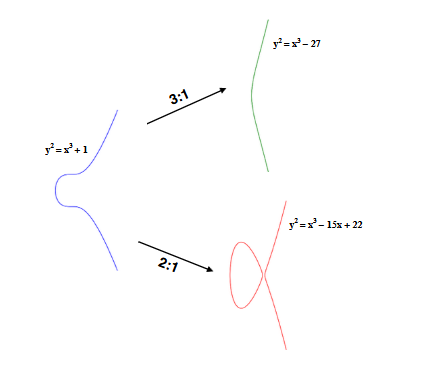
\includegraphics[width=0.5\linewidth]{img/isogeny-example.png}
    \caption{Ejemplo visual de isogenias}
    \label{fig:isogeny-example}
\end{figure}

\subsection{Isogenias duales}

Toda isogenia tiene lo que se denomina una isogenia dual. Estas isogenias se comportan, en mayor parte, como inversas. No técnicamente inversas ya que no son aplicaciones biyectivas, dos isogenias diferentes pueden tener una misma isogenia dual. Esto no tiene mucha repercusión a la hora de trabajar con ellas, ya que la isogenia dual existe y cumple sus propiedades. 

\subsection{Grado de una isogenia}

Al igual que una curva elíptica puede tomar múltiples formas, a la hora de definir una isogenia se puede hacer de miles de formas diferentes. La manera que vamos a tratar nosotros es mediante las fórmulas de Vélu \cite{velu}, que permiten, dada una curva Weierstrass $E$ de dominio y un conjunto finito de puntos $G$, definir una isogenia.

Este conjunto de puntos $G$ serán el kernel de la isogenia, esto es, los puntos cuya imagen será el origen, cuya dimensión definimos como el \textit{grado de la isogenia}. Además, cuando estamos hablando de una isogenia, podemos referirnos a ella como una $k$-isogenia, donde $k$ es su grado.

De esta forma, tenemos que conocer un subgrupo cíclico dentro de una curva dominio va a equivaler conocer una isogenia, su estructura y la curva imagen junto con su estructura de grupo. Las ecuaciones de Vélu nos permitirán pues calcular muy fácilmente todas las isogenias de un grado determinado a partir de una curva origen. Repitiendo el proceso conforme vamos encontrando curvas imagen, obtendremos de manera sencilla todas las isogenias definidas a partir de todas las curvas definidas sobre un mismo cuerpo.

%
%   INVARIANTES
%

\section{$j$-invariantes}

El $j$-invariante de una curva elíptica se puede calcular de varias maneras dependiendo de la forma que tome la curva.

\begin{description}
    \item[Forma de Weierstrass] Dada una curva de la forma $E: y^2 = x^3 + ax + b$, entonces su $j$-invariante se puede calcular mediante
    \[j(E) = 1728 \frac{4a^3}{4a^3 + 27b^2}\]

    \item[Forma de Montgomery] Dada una curva de la forma $E: y^2 = x^3 + ax^2 + x$, entonces su $j$-invariante se puede calcular mediante
    \[j(E) = 256 \frac{(a^2 - 3)^3}{a^2 - 4}\]
\end{description}

Aunque a primera vista uno pueda pensar que este valor va a ser único para cada curva, esto está lejos de la realidad. Por ejemplo, para $\mathbb{F}_{431^2}$ conseguimos un total de $37$ $j$-invariantes.

¿Para qué nos sirve esto? Los $j$-invariantes permiten agrupar las curvas elípticas de un cuerpo. Dos curvas con un mismo $j$-invariantes son isomórficas, lo que significa literalmente que tienen la misma forma. Es decir, desde un punto de vista matemático, dos curvas elípticas con un mismo $j$-invariante se podrían considerar la misma curva, no porque sus ecuaciones sean idénticas sino porque, al existir un isomorfismo entre ellas, sabemos que tienen las mismas propiedades.

Veamos una pequeña aclaración. Trabajando con las ecuaciones de Weierstrass, sean $E,E'$ dos curvas elípticas con el mismo $j$-invariante,

\[ E: y^2 = x^3 + Ax + B \]
\[ E' : y'^2 = x'^3 + A'x' + B' \]

Bajo la asunción que $j(E) = j(E')$ podemos hallar un isomorfismo de la forma $(x,y) = (u^2x', u^3y')$ donde, dependiendo de los valores de $A,B$ tenemos los siguientes valores de $u$

\begin{enumerate}
    \item \textit{Caso $A=0$ $(j=0)$: } $u=(B/B')^{1/6}$
    \item \textit{Caso $B=0$ $(j=1728)$: } $u=(A/A')^{1/4}$
    \item \textit{Caso $AB\neq0$ $(j\neq0)$: } $u=(A/A')^{1/4}=(B/B')^{1/6}$
\end{enumerate}

Mediante este isomorfismo, podremos trabajar con $E$ o $E'$ de forma casi indistinta. Para mayor nivel de detalle, consultar la proposición 1.4 del capítulo III, sección I de \textit{The Arithmetic of Elliptic Curves} de Silverman.

Claramente, a nivel matemático no es lo mismo que a nivel criptográfico. La pregunta entonces es, con lo que respecta a SIKE, ¿dos curvas con el mismo $j$-invariante son la misma? Pues depende del momento. Ya lo veremos con más detalle más adelante pero en un momento del intercambio de clave tenemos que calcular la imagen de unos puntos, por lo que ahí claramente no podemos considerar cualquier curva isomórfica como la misma, ya que nos interesa su valor concreto. Sin embargo, a la hora de encriptar un mensaje, utilizamos el $j$-invariante de la curva compartida el cual como acabamos de ver se mantiene entre isomorfismos.

Podríamos pensar que reducir tan drásticamente el número de valores es un contratiempo para nuestro protocolo, por el contrario, aunque el número de valores parece que desciende, las isogenias disponibles siguen siendo las mismas. Mediante nuestro protocolo nos interesa cambiar de $j$-invariante, más que de curva, ya que como acabamos de ver podríamos no haber hecho ninguna operación efectiva, matemáticamente.

%
%   GRAFOS DE ISOGENIAS
%

\section{Grafos de isogenias}

Una isogenia puede calcularse de mil maneras diferentes, la forma que utilizaremos define previamente el kernel de la isogenia y a partir de este y la curva dominio obtenemos la isogenia y la curva imagen. Siendo una isogenia cualquier morfismo 

\[\phi : E \to E'\]
\[\text{con }Ker(\phi) = K\] 

la curva imagen $E'$ suele ser definida como $E/K$, resultando en la siguiente ecuación

\[\phi : E \to E/K\]

que definiría exactamente la misma isogenia que la que hemos definido antes.

A partir de los $j$-invariantes, el orden de nuestro kernel y las fórmulas de Vélu \cite{velu}, tomando un primo $l$ diferente a nuestro primo $p$, podemos generar un grafo con las $l$-isogenias  entre los $j$-invariantes.

Este grafo tendría como nodos los $j$-invariantes y como aristas las mismas $l$-isogenias. Este grafo no sólo es útil computacional y matemáticamente sino que permitirá mostrar visualmente cómo funciona el protocolo de intercambio de claves de una forma muy intuitiva.

\subsection{Creación del grafo}

Veamos cómo creamos, paso a paso, un grafo de isogenias. Tomemos de punto de inicio el primo $p=431$, el cuerpo con el que vamos a trabajar entonces es $\mathbb F_{431^2}$.

Empezamos con una curva elíptica $E_0: y^2 = x^3 + (208i+161) x^2 + x$. Calculamos su $j$-invariante para una curva Montgomery y tenemos que 

\[j(E_0) = 256 \frac{((208i+161)^2 - 3)^3}{(208i+161)^2 - 4} = 364i+304 \]

Y de aquí obtenemos el primer nodo de nuestro grafo.

\begin{figure}[!ht]
    \centering
    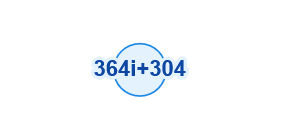
\includegraphics[width=0.33\linewidth]{img/isogeny-graph-step-1.png}
    \caption{Primer nodo del grafo}
    \label{fig:isogeny-graph-step-1}
\end{figure}

Una vez tenemos ya el primer nodo, vamos a seguir completando el grafo. A partir de nuestra curva $E_0$ vamos a tomar la $2$-isogenia

\[ \phi : E_0 \to E_1 \]
\[ \phi : x \mapsto \frac{x((350i + 68)x - 1}{x - (350i + 68)} \]

donde $E_1$ es la curva Montgomery $E_1 : y^2 = x^3 + (102i+423)x^2 + x$. Calculamos el $j$-invariante de $E_1$ y obtenemos que

\[j(E_0) = 256 \frac{((102i+423)^2 - 3)^3}{(102i+423)^2 - 4} = 344i+190 \]

Tenemos ya dos nodos y una arista en nuestro grafo.

\begin{figure}[!ht]
    \centering
    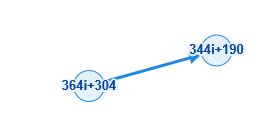
\includegraphics[width=0.5\linewidth]{img/isogeny-graph-step-2.png}
    \caption{Añadimos la primera arista al grafo}
    \label{fig:isogeny-graph-step-2}
\end{figure}

Sin embargo, a la hora de visualizar las aristas, aunque deberían ser dirigidas como lo acabamos de ver, vamos a tratar con un grafo no dirigido ya que, al existir las isogenias duales, se entiende que si existe una arista en una dirección, necesariamente existirá una en sentido contrario.

\newpage\begin{figure}[!ht]
    \centering
    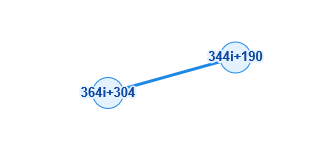
\includegraphics[width=0.5\linewidth]{img/isogeny-graph-step-3.png}
    \caption{Grafo no dirigido}
    \label{fig:isogeny-graph-step-3}
\end{figure}

Completando el grafo, llegaremos al siguiente grafo

\begin{figure}[!ht]
    \centering
    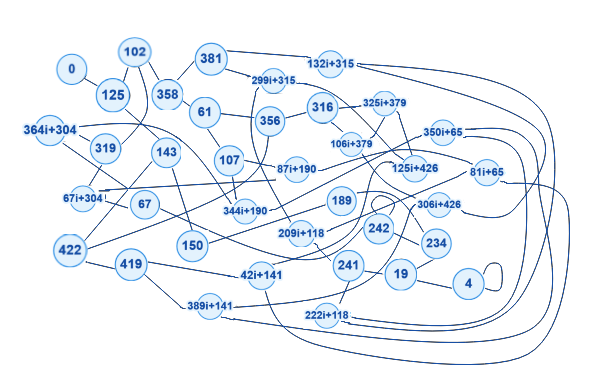
\includegraphics[width=1\linewidth]{img/isogeny-graph.png}
    \caption{Grafo de $2$-isogenias para $p=431$}
    \label{fig:isogeny-graph}
\end{figure}
